%!Mode::"TeX:UTF-8"

\documentclass[UTF8,adobefonts]{ctexart}

\title{基于压缩后缀数组的短读序列比对算法}
\author{李双江}
\date{June 2014}

\usepackage{natbib}
\usepackage{graphicx}
\usepackage{CJKutf8}
\usepackage{lineno}
\usepackage{indentfirst}
\usepackage[unicode]{hyperref}
\usepackage{amsmath}
\usepackage{amsthm}
\usepackage{amssymb}
\usepackage{algorithm}
\usepackage{algorithmicx}
\usepackage[noend]{algpseudocode}
\usepackage{multirow}


\newtheorem{theorem}{定理}[section]
\newtheorem{lemma}{引理}[section]
\newtheorem{definition}{定义}[section]
\newtheorem{corollary}[theorem]{推论}
\renewcommand{\proofname}{\bf 证明}


\floatname{algorithm}{算法}
\renewcommand{\algorithmicrequire}{\textbf{Input:}}
\renewcommand{\algorithmicensure}{\textbf{Output:}}

\graphicspath{{figures/}}

% set margin with left:3cm,right:2cm,up:3cm,down:2cm
\oddsidemargin 1.46 true cm
\evensidemargin -0.54 true cm
\topmargin -0.54 true cm
\headheight 12.9pt
\headsep 17.3527pt
\textheight 24.2 true cm
\textwidth 15 true cm
\footskip 0.5 cm
\parskip 0.5ex plus 0.25ex minus 0.25ex

\begin{document}
\maketitle
\pdfbookmark[3]{bookmark text}{anchor name}

\section{引言}

随着生物学,医学等相关科学的发展,新的DNA测序技术不断涌现,其中,以Illumina/Solexa为代表的NGS(NEXT-GENERATION SEQUENCING DAT)
技术以其低廉的测序成本成为当前的主流DNA测序技术。NGS测序的每一次
测序实验都会得到大量的短读(short reads)序列(5亿到20亿个)。在对测序得到的数据做下一步分析研究前,首先要对短读进行重组(assembly)
或者比对(alignment),这也对应着从头测序和重测序两种常见的测序。重测序实验中得到的短读中每一个短读一般不超过1000个碱基,
,但数量巨大。短读比对的的目标是把测序实验中得到的大梁短读映射到一个参考序列
上去,参考序列一般选择已经测序的基因组,如人类基因组等。映射的过程是对每一个短读在参考序列上查找一个合适的位置,使得短读在该
位置和参考序列尽量匹配。

综上所述,短读序列的映射问题可以抽象为一个模式查找问题:给定一个共有$m$个模式的模式集合$P=\{P_1,P_2\ldots P_m\}$,每个
模式的长度已知分别为$l_1,l_2\ldots l_m$,已知一个长为$n$的参考序列$T$,求得一个集合$S=\{s_1,s_2\ldots s_n\}$使得$P_i=T_{s_i\ldots s_i+l_i-1}$。
这个查找的过程即为短读到参考序列的比对映射。其中参考序列$T$和短读序列$P_i$都是由DNA测序中常用的碱基字符$\{A,T,C,G,U,N\}$
构成的。

为实现快速且准确的短读序列映射,近年来出现了很多比对算法。所有这些算法都可以分为两类,一类是通过对短读序列使用散列表等方法建
立短读序列的索引,之后遍历整个参考序列。另一类是为参考序列建立索引,之后再对每个短读进行独立的比对。

第一类比对算法的代表是MAQ,ZOOM,SHRiMP等。MAQ\cite{li2008mapping}基于散列技术,结合短读中每一个核苷酸的测序质量分数,实现了
无空位(ungapped)比对。ZOOM\cite{lin2008zoom}使用了space seeds技术,提高了比对的精确率。而SHRiMP\cite{rumble2009shrimp}则结合space seeds''
和smith-waterman算法得到了更高的精确率。

第二类算法为参考序列建立索引,通过索引后的数据可以实现快速的比对。如SOAP,WHAM,BFAST等。SOAP\cite{li2008soap}使用seeds技术
和一个散列查询表加速比对,且可以处理较少的空位比对。WHAM\cite{li2012wham}对参考序列建立散列表,先通过散列表查找潜在的比对
位置,再进一步比对确定最终结果。BFAST\cite{homer2009bfast}则通过
为参考序列建立多个索引来提高精确度。这几种方法使用的索引方法都需要很大的内存空间,所以比对时空间需求很大,尤其是在用类基因
组这样的较大序列作为参考序列时。在第二类方法中以SOAP2,Bowtie,BWA为代表的基于BW变换(Burrows-Wheeler transform,BWT)\cite{ferragina2005indexing}来创建参考序列
索引的方法具有很大的空间优势。Bowtie\cite{langmead2009ultrafast}使用BWT建立索引,采用回溯递归
的搜索方法,再结合双端搜索实现了高速,空间高效的比对,是目前最快的比对软件之一,但缺陷是不能实现空位(gap)比对。BWA\cite{li2009fast}
也是基于BWT的一种比对算法,比对速度较Bowtie慢,但可实现空位比对。SOAP2\cite{li2009soap2}使用了bidirectional BWT来建立参考序列
的索引,比对速度和Bowtie相当。基于BWT的这些方法都使用了后向搜索方法\cite{lippert2005space}来加速查询。后向搜索可以在$O(m)$时间内实
现长为$m$的字符串的计数查询,以及$O(m\log n)$时间复杂度的query查询。利用后向搜索的性质,Bowtie实现了基于
回溯法的非精确匹配算法,而BWA则采用前缀树搜索的方法实现非精确匹配。在实现非精确匹配的基础上,加上一些打分机制,既实现了短读
序列到参考序列的匹配。

本文提出的CSAA(csa alignment)采用压缩后缀数组(Compressed Suffix Array,CSA)\cite{grossi2005compressed}索引参考序列,利用后向搜索的方法实现短
读比对算法。这一算法的核心是用CSA的后向搜索结合优先队列实现近似搜索,从而支持短读比对,且支持gap比对。CSAA中后向搜索实现快速搜索,
优先队列保存所有的匹配位置,并为每个匹配位置打分,在匹配过程中,通过分支限界抛弃所有低分搜索方向,降低搜索空间,
同时保证匹配结果最优。按照上一节中对短读比对算法的分类,该算法属于对参考序列进行索引的比对算法。

\section{Definitions and notations}

\subsection{后缀数组和压缩后缀数组}
压缩后缀数组(CSA)是由Grossi和Vitter\cite{grossi2005compressed}最早提出的第一种实现全文索引的压缩索引数据结构,是对后缀数组(SA)
\cite{manber1993suffix}占用空间过大的改进,并且实现了自索引特性。

设长为$n$的文本序列$T$,字符集为$\Sigma$,本文中将假设$T$有一个特殊的结尾符号$\$$,$\$$不在$\Sigma$中并且字典序小于$\Sigma$
中的所有符号。假设$T$存储在一个数组$T[0\ldots n-1]$中。对任何的整数$i$,假设

\begin{itemize}
    \item $T[i]$为$T$中从左往右0开始的第$i$个字符;
    \item $T_i$为$T$的第$i$个后缀,即$T_i=T[i]T[i+1]\ldots T[n-1]$。
\end{itemize}

$T$的后缀数组$SA[0\ldots n-1]$定义为
$T$的$n$个后缀按字典序排序后的序列,由$\{0,1,\ldots, n-1\}$的一个排列构成,满足$T_{SA[0]}<T_{SA[1]}<\ldots<T_{SA[n-1]}$。即$SA[i]$
表示$T$的$n$个后缀中第$i$小的后缀的开始位置。如表\ref{tab:tabsuffix}所示。后缀数组占用空间$n\log n$,给定文本$T$和其后缀数组
$SA[0\ldots n-1]$,$T$中的任何模式$P$可以在$O(|p|\log n+occ)$时间复杂度内求出其出现位置\cite{manber1993suffix},并且不需要
读原文本$T$。其中$occ$是模式的出现次数。

对于任意的整数$i \in [0\ldots n-1]$,定义$SA^{-1}[i]=j$使得$SA[j]=i$,很明显$SA^{-1}[i]$为$T_i$在$T$的所有后缀中的排名,即
$T$的后缀中比$T_i$小的后缀的数量。

\begin{table}[htbp]
    \caption{$acaaccg\$$的后缀数组和$\Phi$数组}
    \label{tab:tabsuffix}
    \centering
    \begin{tabular}{lllllll}
        \hline\\
%        \toprule
        $i$&$T[i]$&$T_i$&$SA[i]$&$T_{SA[i]}$&$\Phi[i]$&$T[SA[i]]$\\
        \hline\\
%        \midrule
        0&a&acaaccg\$&7&\$&2&\$\\
        1&c&caaccg\$&2&aaccg\$&3&a\\
        2&a&aaccg\$&0&acaaccg\$&4&a\\
        3&a&accg\$&3&accg\$&5&a\\
        4&c&ccg\$&1&caaccg\$&1&c\\
        5&c&cg\$&4&ccg\$&6&c\\
        6&g&g\$&5&cg\$&7&c\\
        7&a&\$&6&g\$&0&g\\
        \hline
%        \bottomrule
    \end{tabular}
\end{table}

\begin{equation}\label{eq:phi}
    \Phi [i] = j \qquad if\ SA[j] = (SA[i]+1)\mod n \cite{huo2014practical}
\end{equation}

序列 $T$ 的压缩后缀数组(Compressed Suffix Array, CSA)是对后缀数组(SA)空间复杂度过大的一个改进。其本身也是一个包含$n$个
整数与后缀数组$SA$大小相同且由$SA$的近邻函数变换而来的数组$\Phi$。近邻函数定义如\ref{eq:phi},由于$T[n-1]=\$$,所以
$\Phi[0]=SA^{-1}[0]$。另一个角度来看,若后缀$T_k$在$T$的后缀中排名为$i$,则$\Phi[i]$为后缀$T_{k+1}$在$T$的后缀中的排名。
同时,可以看到$SA^{-1}[1]=SA^{-1}[SA[SA^{-1}[0]+1]=\Phi[\Phi[SA[SA^{-1}[0]]]]=\Phi[\Phi[0]]$,同理可以得到$SA^{-1}[2]=\Phi[\Phi[\Phi[0]]]$。
以此类推,即可根据$\Phi[0\ldots n-1]$迭代求出$SA^{-1}[0\ldots n-1]$,由$SA^{-1}[0\ldots n-1]$可快速求出$SA[0\ldots n-1]$。
由此可得出,从后缀数组$SA[0\ldots n-1]$到数组$\Phi[0\ldots n-1]$的变换是可逆的。

$\Phi[0\ldots n-1]$包含$n$个整数,显示存储时,也需要$n\lceil \log n \rceil$位的存储空间,同后缀数组$SA$相同。然而,观察表\ref{tab:tabsuffix}
可以发现$\Sigma[1\ldots n-1]$可以分解为$|\Sigma|$个严格递增的序列,这使得压缩后缀数组可以用简明数据结构存储。而$\Sigma[1\ldots n-1]$
的递增属性则是基于以下引理。

\begin{lemma}\label{ref:lem1}
对于任意的整数$i<j$,若$T[SA[i]]=T[SA[j]]$,则$\Phi[i]<\Phi[j]$。
\end{lemma}

\begin{proof}
    当$i<j$时,则$T_{SA[i]}<T_{SA[j]}$一定成立,反之亦然。这等价于当$T[SA[i]]=T[SA[j]]$时,$T_{SA[i]+1}<T_{SA[j]+1}$,即$T_{SA[\phi[i]]}<T_{SA[\Phi[j]]}$,
    所以可以得到$\Phi[i]<\Phi[j]$。即引理\ref{ref:lem1}成立。
\end{proof}

对任意一个$\Sigma$中的字符$c$,定义$\alpha(c)$为$T$的后缀中首字符小于$c$的后缀的数目,定义$\beta(c)$为$T$的后缀中首字符为
$c$的后缀的数目。则有以下结论:

\begin{corollary}\label{cor1}
对于$\Sigma$中的任意一个字符$c$,$\Phi[\alpha(c)], \Phi[\alpha(c)+1] \ldots \Phi[\alpha(c)+\beta(c)− 1]$是一个严格递增序列。
\end{corollary}

\begin{proof}
    对于任意的字符$c$,$T[SA[\alpha(c)]]=T[SA[\alpha(c)+1]]=\ldots =T[SA[\alpha(c)+\beta(c)-1]]=c$,由引理\ref{ref:lem1}可知,
    $\Phi$在$\Phi[\alpha(c)\ldots \alpha(c)+\beta(c)-1]$上严格递增。
\end{proof}

根据以上结论,$\Phi$可以划分为$|\Sigma|$个递增序列,这个递增性质是压缩后缀数组可压缩性的本质保证。Grossi和Vitter\cite{grossi2005compressed}
据此提出了一种压缩模式来存储$\Phi$,使得可以在$O(n(H_0+1))$位的空间内存储$\Phi$数组,其中$H_0 \leq \log |\Sigma|$,是文
本$T$的0阶经验熵。

\subsection{后向搜索}

压缩后缀数组上的后向搜索模式匹配算法是由Sadakan最早提出来的\cite{sadakane2002succinct}。如上文中所述,我们用$(l,r)$
表示一个模式串在$T$上的后缀位置,模式匹配的目的正是要找到$P$的$(l,r)$。首先,计算$P[m]$的后缀位置,很明显$(\alpha(P[m]),
\alpha(P[m])+\beta(P[m])-1)$就是。假设一般情况,我们已经知道$P[i+1\ldots m-1]$的后缀数组位置为$(l_{P_{i+1}},r_{P_{i+1}})$,
那么$P[i\ldots,m-1]$的后缀数组位置$(l_{P_i},r_{P_i})$必定是由$P[i]$的后缀数组位置的一部分组成的,设$P[i]$的后缀数组位置
为$(l_{P[i]},r_{P_i})$,那么对于$l_{P[i]\leq k \leq r_{P_i}}$只要$SA^{-1}SA[k]+1$在$(l_{P_{i+1}},r_{P_{i+1}})$中,$k$一定在$(l_{P_i},r_{P_i})$
中。也就是说$P[i\ldots n-1]$的出现位置一定是$P[i]$的出现位置后面紧跟着$P[i+1\ldots m-1]$的出现位置。加上$\Phi[i]=SA^{-1}[SA[i]+1]$,
所以我们可以得到公式\ref{equa:equa1}。

\begin{equation}\label{equa:equa1}
    k \in (l_{P_i},r_{P_i}) \iff k \in (l_{P[i]},r_{P[i]}) \wedge \Phi[k] \in (l_{P_{i+1}},r_{P_{i+1}})
\end{equation}

由于在简明数据结构存储下$\Phi$可以在常数时间内获得,并且其值在$(l_{P_{i+1}},r_{P_{i+1}})$上是递增的,所以,可以用二分搜索
来搜索$\Phi[k]$是否在$(l_{P_{i+1}},r_{P_{i+1}})$上,时间复杂度是$O(\log n)$。重复上述过程$m$次,即可在CSA上用$O(m\log n)$
时间复杂度找到模式$P[0\ldots m-1]$的后缀数组范围$(l,r)$

算法\ref{alg:backwardsearch}给出了CSA上的后向搜索的伪代码。而图\ref{figbackwardsearch}给出了一个采用算法\ref{alg:backwardsearch}
的例子,搜索模式$P=CCAGTA$。每一个方块儿对应一个字符的后缀数组区域,灰色的区域表示对应$P$的一个后缀在$T$的后缀数组上的位置
范围。在右起第二步,计算新的区域时,根据下一个字符$G$的后缀范围,计算其$\Phi$值,查看这个$\Phi$是否落在当前模式$TA$的后缀范
围内,由于$\Phi$的递增特性,很容易用二分搜索方法找到新的区域的上下界。

\begin{algorithm}
    \caption{后向搜索}
    \label{alg:backwardsearch}
    \begin{algorithmic}[1]
        \Require $P,\Phi,\alpha,\beta$
        \Ensure $(l,r)$
        \Function{backwardSearch}{$P,\Phi,\alpha,\beta$}
        \State $l_{m} \gets 0;r_{m}\gets n-1$
        \For {$i\gets m-1$ down to $0$}
            \State $l_i \gets \min\{ k \in [\alpha(P[i]),\alpha(P[i])+\beta(P[i])-1],\Phi[k] \in [l_{i+1},r_{i+1}]\}$
            \State $r_i \gets \max\{ k \in [\alpha(P[i]),\alpha(P[i])+\beta(P[i])-1],\Phi[k] \in [l_{i+1},r_{i+1}]\}$
            \If{$l> r$}
                \State \Return $\varnothing$
            \EndIf
        \EndFor
        \State \Return $(l_0,r_0)$
        \EndFunction
    \end{algorithmic}
\end{algorithm}


\begin{figure}[t]
    \centering
    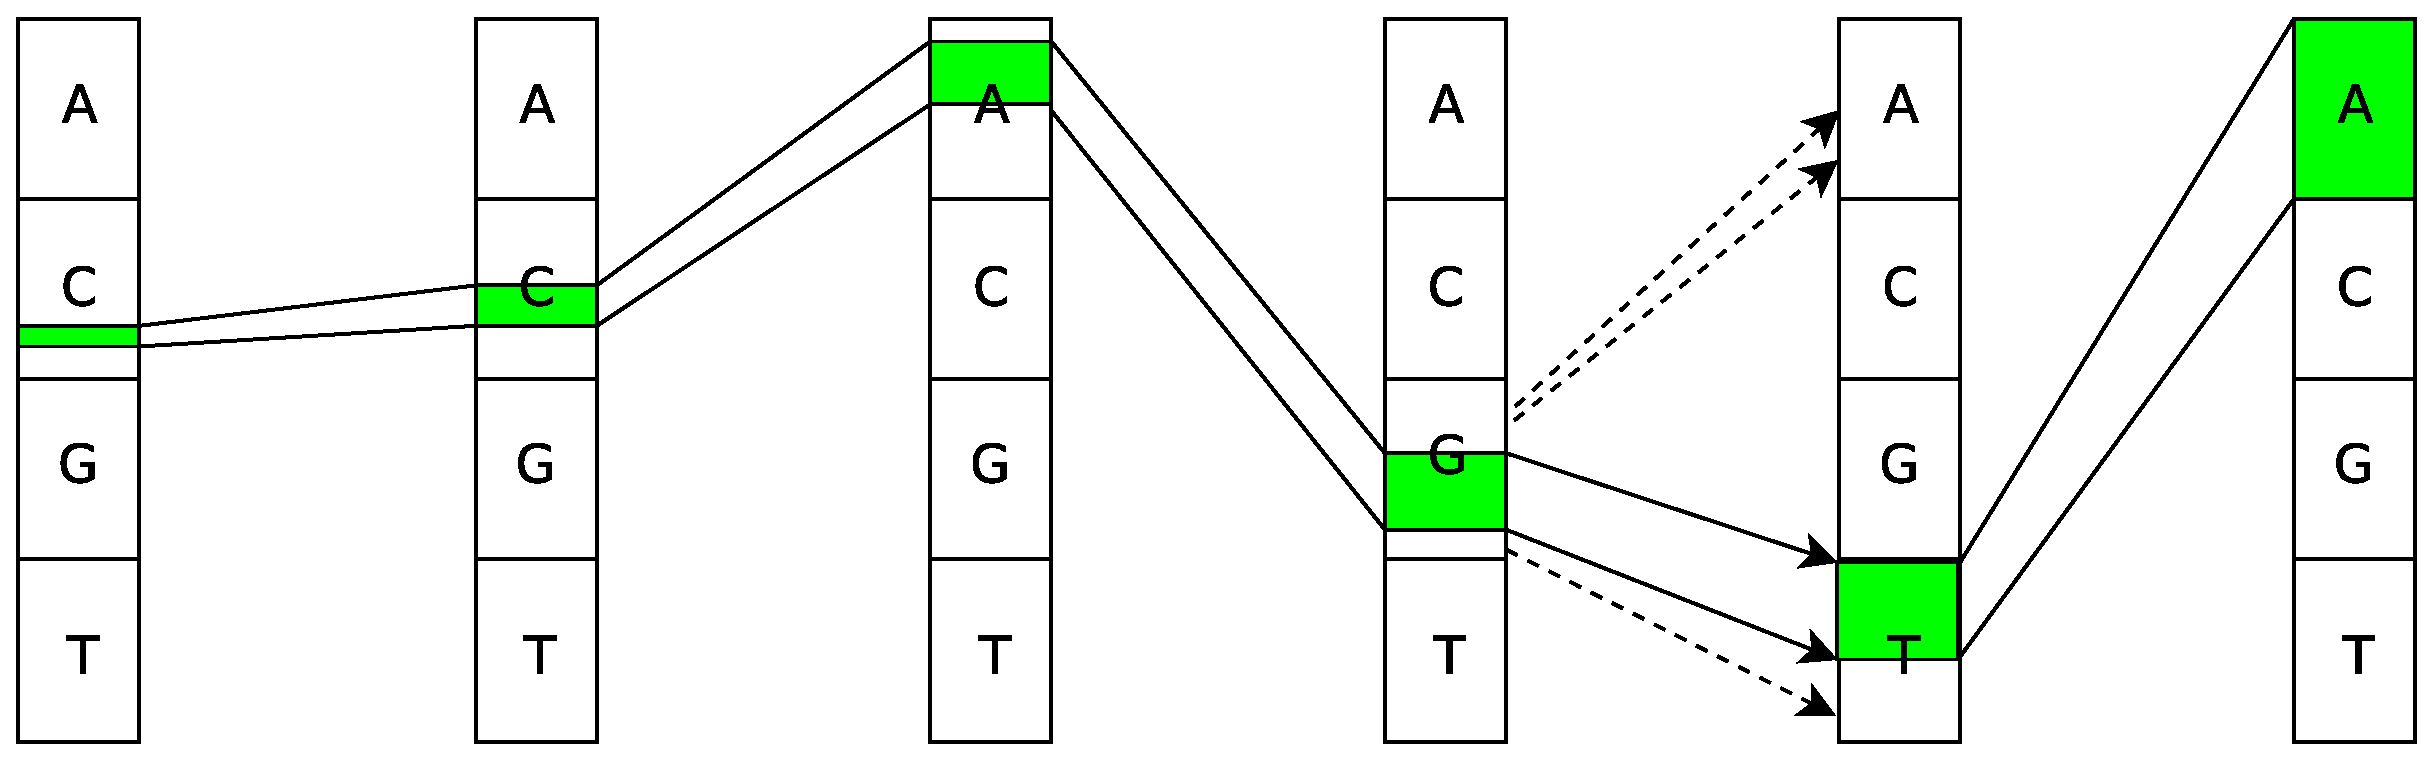
\includegraphics[width=0.7\textwidth]{csa_backwardsearch}
    \caption{CSA上的后向搜索}
    \label{figbackwardsearch}
\end{figure}

\subsection{CSA索引}

压缩后缀数组有两个基本特征:$\Phi$数组的递增特性以及算法\ref{alg:backwardsearch}中的后向搜索。前者保证了通过特定的编码
可以实现压缩后缀数组的压缩性质,后者则保证了压缩后缀数组对文本的检索能力。本文中使用的压缩后缀数组索引是用gap编码实现压缩存储,
使用后向搜索做匹配搜索的一种全文压缩索引。索引只需一次建立,即无需再保存庞大的参考序列数据,并且一次建立可以多次使用,而且
空间利用率最高。

\section{CSA短读比对算法}

CSA短读比对算法(CSAA)采用CSA索引参考序列,利用CSA的后向搜索完成匹配过程。CSA的后向搜索是一种精确匹配算法,由于
DNA序列存在变异,以及测序技术有一定的错误率,所以不能简单的使用精确搜索算法。本文提出了两种策略来实现短读比对中的非精确匹配
要求。一是在后向搜索过程中引入了搜索树,使得在搜索过程中可以随时对短读序列进行插入,删除,替换等操作。另一种策略是
采用类似优先队列的数据结构,这一数据结构结合打分机制保证在后向搜索的每一步中都是沿着最优的搜索方向前进,并且采用分支限界
的策略适时淘汰很差的搜索方向。

\subsection{精确匹配}
精确匹配本质上就是是后向搜索。根据算法\ref{alg:backwardsearch},可知给定一个长为$n$的参考序列$T$,$P$为测序得到的短读序列中的
一个短读,假设已经获取到短读的后缀$P[i+1\ldots m-1]$的后缀数组位置$(l_{P_{i+1}},r_{P_{i+1}})$,那么可以跟据公式\ref{equa:exac}
确定后缀$P[i\ldots m-1]$的后缀数组位置$(l_{P_i},r_{P_i})$。

\begin{equation}\label{equa:exac}
    \begin{split}
        l_{P_i} \gets &\min\{ k \in [\alpha(P[i]),\alpha(P[i])+\beta(P[i])-1],\Phi[k] \in [l_{P_{i+1}},r_{P_{i+1}]}\}\\
        r_{P_i} \gets &\max\{ k \in [\alpha(P[i]),\alpha(P[i])+\beta(P[i])-1],\Phi[k] \in [l_{P_{i+1}},r_{P_{i+1}]}\}
    \end{split}
\end{equation}

由于$\Phi[\alpha(P[i])\ldots \alpha(P[i])+\beta(P[i])-1]$是严格递增序列,所以公式\ref{equa:exac}可以采用二分搜索实现。
搜索$[\alpha(P[i],\alpha(P[i])+\beta(P[i])-1]$的
左边界和右边界在$\Phi[\alpha(P[i])\ldots \alpha(P[i])+\beta(P[i])-1]$上是否出现,即可得$P[i\ldots n-1]$的后缀数组
位置$(l_{P_i},r_{P_i})$。

综上所述,可以得到以下精确匹配算法\ref{alg:exac},该算法采用后向搜索的方法,根据一个给定的模式$X$的后缀数组$(l,r)$和
字符$c$计算出新模式$cX$的后缀数组位置。根据这个算法,加上一定策略,即可得到我们下文将提出的近似匹配算法。

\begin{algorithm}
    \caption{精确匹配}
    \label{alg:exac}
    \begin{algorithmic}[1]
        \Require $\Phi,\alpha,\beta,l_{old},r_{old},c$
        \Ensure $(l,r)$
        \Function{ExactMatch}{$\Phi,\alpha,\beta,l_{old},r_{old},c$}
        \State $l_c \gets \alpha(c)$
        \State $r_c \gets \alpha(c)+\beta(c)-1$
        \State $(l,r) \gets $\Call{binarySearch}{$\Phi[l_c\ldots r_c],l_{old},r_{old}$}
        \If{$l>r$}
            \State \Return $\varnothing$
        \Else
            \State \Return $(l,r)$
        \EndIf
        \EndFunction
    \end{algorithmic}
\end{algorithm}

\subsection{近似匹配}

根据上一小节所述的精确匹配算法思想,模式匹配就只有两种结果,要么匹配上,要么没匹配上这种完全的匹配方式并不适合大多数存在变异
和测序误差的短读序列。本文提出的CSAA算法是建立在非精确匹配的基础上的。

由于同一物种之间存在的个体差异(具体在DNA上表现为单核苷酸变异SNP),以及测序技术存在的误差,Resequencing技术得到的短读序列和
该物种的标准参考序列之间哪怕是同一基因片段也必然存在着一些不同,这会造成即使同一种基因序列也无法完全比对映射到参考序列上。
所以对短读和参考序列之间的比对仅仅精确比对映射是远远不够的,这会造成大量的短读因为和参考序列相差一两个核苷酸不同而不能映射
到参考序列上,而这一两个不同的核苷酸很可能是测序误差或者生物个体之间的SNP造成的,不应当认为二者是不能匹配的。所以,采用合适
的非精确比对算法是必须的。本文提出的非精确匹配算法中,支持对短读进行替换(substitude),插入(insert),删除(delete)三种变换操
作,通过这三种操作可以保证变异的或者发生测序错误的短读序列依然能正确匹配到参考序列的合适位置上。

考虑一个给定的长为$m$的短读序列$P$,采用后向搜索,当搜索到第$i+1$个位置时,得到序列$P_{i+1}$的后缀数组位置$(l_{i+1},r_{i+1})$,
依照精确匹配的算法下一步应当在$(l_{i+1},r_{i+1})$的基础上搜索字符$P[i]$,从而得到一个新的后缀数组位置$(l_i,r_i)$。在此,如果我们不
搜索$P[i]$,而是搜索另一个符号$c \neq P[i]$,得到另一个后缀数组位置$(l_{i}^{'},r_{i}^{'})$。接着在$(l_{i}^{'},r_{i}^{'})$基础
上继续搜索$P[0\ldots i-1]$,那么最终得到后缀数组位置$(l_0,r_0)$将不再是序列$P$的一个后缀数组位置了,而是将$P[i]$替换为$c$
后的新字符串的后缀数组位置。称这个新位置为$P$的一个替换近似串的后缀数组位置,计为$(l_0,r_0,m,P(S_i))$,即长为$m$的序列$P$在
$i$位置进行一次替换后可以映射到参考序列的后缀数组位置$(l_0,r_0)$。

图\ref{fig:substitude}给出了把短读序列中的一个符号$T$替换为$A$时的搜索过程,实线为精确匹配的过程,虚线是替换后的搜索过程。

\begin{figure}[htbp]
    \centering
    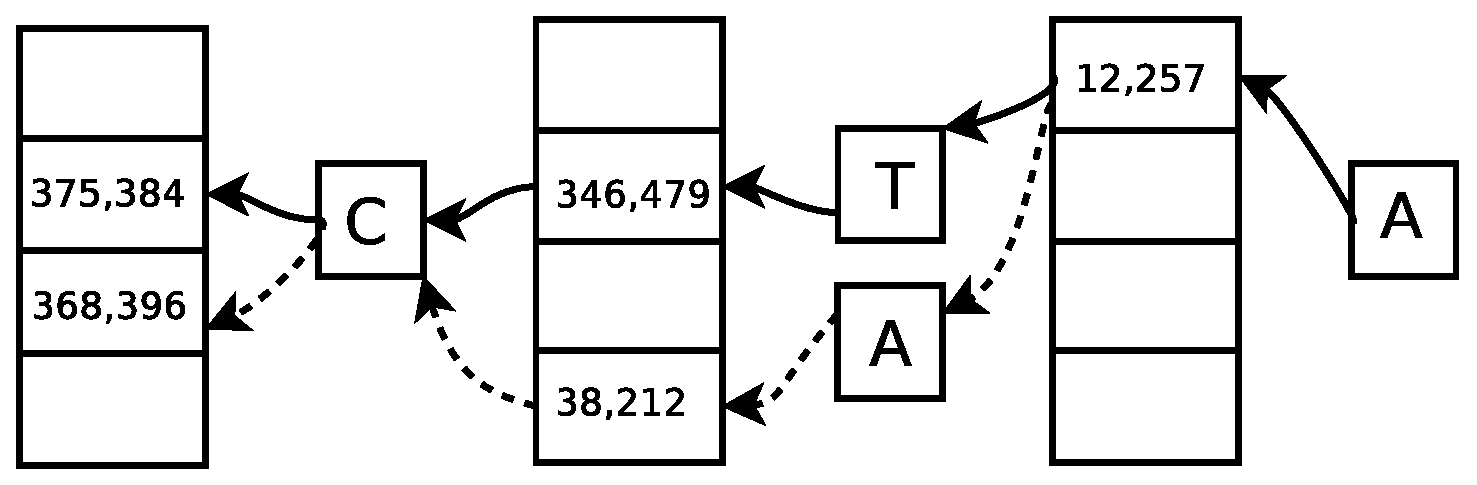
\includegraphics[width=0.7\textwidth]{substitude.eps}
    \caption{替换操作示例} \label{fig:substitude}
\end{figure}

不同于替换操作,如果在搜索到$P[i]$时,放弃搜索$P[i]$符号,直接在$(l_{i+1},r_{i+1})$的基础上搜索序列$P[0\ldots i-1]$,那么
最终得到的后缀数组位置$(l_0,r_0)$将是$P$删除$P[i]$后的近似串在参考序列上的后缀数组位置,计为$(l_0,r_0,m,P(D_i))$,,即长为$m$
的序列$P$在$i$位置进行一次删除后可以映射到参考序列的后缀数组位置$(l_0,r_0)$。

如图\ref{fig:delete}所示为删除短读序列中的一个符号后的搜索过程。

\begin{figure}[htbp]
    \centering
    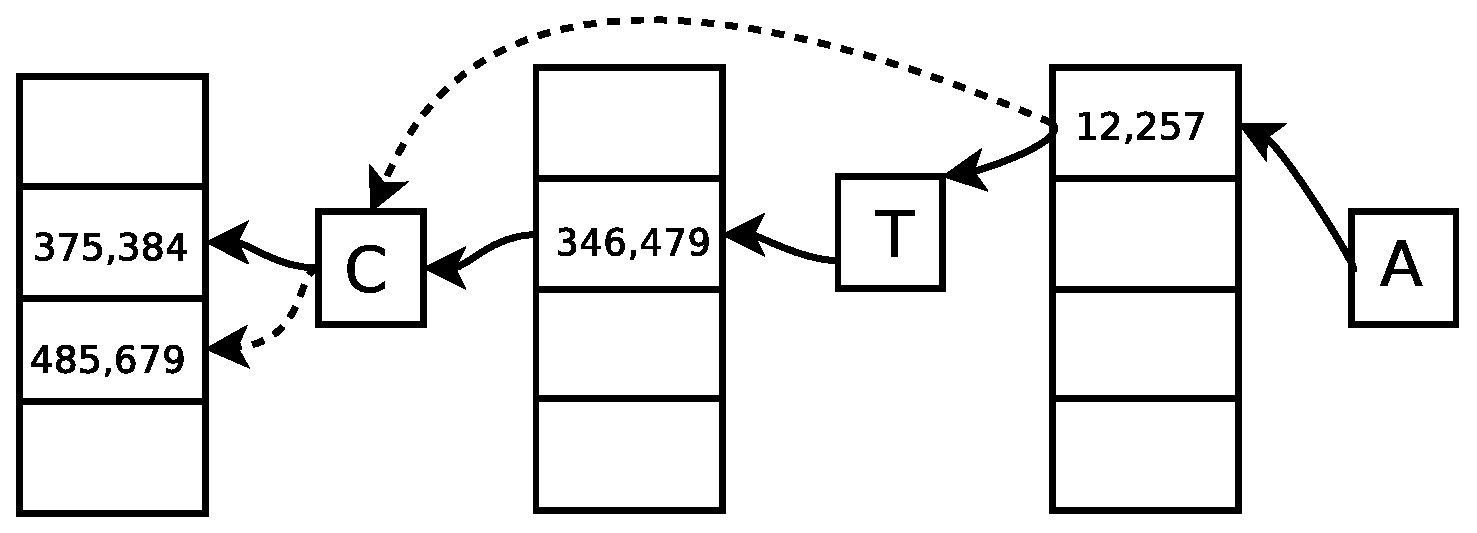
\includegraphics[width=0.7\textwidth]{delete.eps}
    \caption{删除操作示例} \label{fig:delete}
\end{figure}

对于插入操作,在搜索到$P[i]$时,不直接搜索$P[i]$,而是在$l_{i-1},r_{i-1}$的基础上搜索符号$c$,得到$(l_{i}^{'},r_{i}^{'})$,接着
在此基础上搜索序列$P[0\ldots i]$,最终得到的后缀数组位置$(l_0,r_0)$将是$P$在$i$位置插入符号$c$后的近似序列的后缀数组位置。计为
$(l_0,r_0,m,P(Ii)$,即长为$m$的序列$P$在$i$位置插入一个符号后可以映射到参考序列的后缀数组位置$(l_0,r_0)$。

如图\ref{fig:insert}所示为插入一个符号'A'前后的短读序列中的一个符号后的搜索过程。

\begin{figure}[htbp]
    \centering
    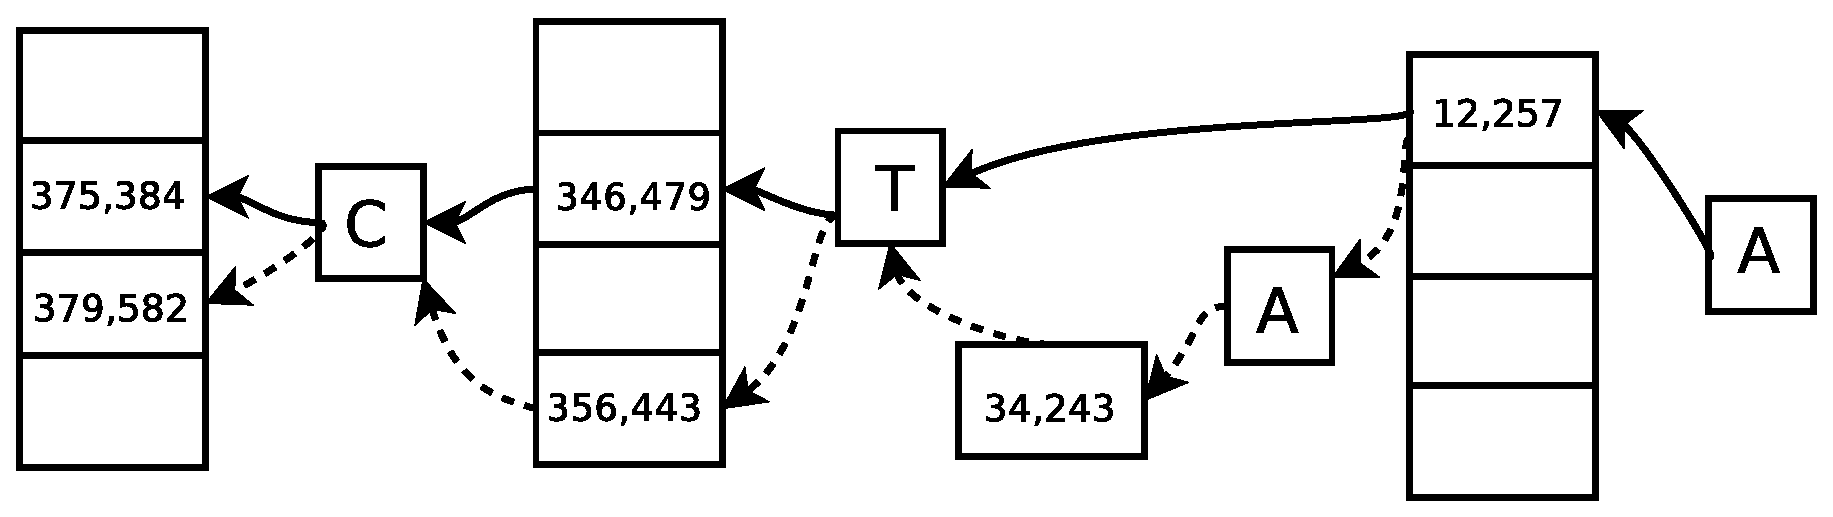
\includegraphics[width=0.7\textwidth]{insert.eps}
    \caption{插入操作示例} \label{fig:insert}
\end{figure}

综上所述,通过在搜索的过程中加入替换,删除,插入三种操作,可以扩展后向搜索的搜索方向,达到近似匹配的目的。如果已知模式串的
某个字符是不可靠的,那么我们可以通过在这个位置加入上述三种操作,实现非精确匹配,查找到这个模式串的可能匹配位置。而大多数情况
下,我们是不知道具体哪一个字符不可靠的,所以只能试探每一个字符,对每一个字符都做删除,替换,插入操作,从而找到一个合适的位置。
据此,我们提出非精确匹配算法\ref{alg:inexact},这个算法递归的实现近似匹配,对$P$的每一个位置都做了三种操作,所以这个算法的本
质是对长为$m$的序列$P$做了所有可能的近似串的搜索,即做了$|\Sigma|^m$个序列的匹配。因为采用了后向搜索的过程,每一次递归实际都
是产生$\Sigma$次替换递归,$\Sigma$次插入递归,和1次删除递归,所以实际的时间复杂度
满足递归式\ref{equa:exact}。解递归式\ref{equa:exact}可得$T(m)=(2\Sigma+1)^{m-1}+\Theta(m\log n)$。
\begin{equation}\label{equa:exact}
    T(m)=\begin{cases}\Theta(1) & \mbox{if } m=1 \\
    2(\Sigma+1)T(m-1)+\Theta(\log n) & \mbox{if } m>1\end{cases}
\end{equation}

\begin{algorithm}
    \caption{近似匹配}
    \label{alg:inexact}
    \begin{algorithmic}[1]
    \Require $\Phi,\alpha,\beta,l,r,P,i$
    \Ensure $(l,r)$
    \Function{inexactMatch}{$\Phi,\alpha,\beta,l,r,P,i$}
    \If{$i<0$}
    \State \Return $(l,r)$
    \EndIf
    \State $S \gets \varnothing$
    \State $S \gets S\ \cup$\ \Call{inexactMatch}{$\Phi,\alpha,\beta,l,r,P,i-1$} \Comment{删除$P[i]$操作}
    \ForAll{$c \in \Sigma$}
    \State $(l,r)\gets$\Call{ExacMatch}{$\Phi,\alpha,\beta,l,r,c$} \Comment{调用算法\ref{alg:exac}}
        \If{$l\leq r$}
        \State $S \gets S\ \cup\ $ \Call{inexactMatch}{$\Phi,\alpha,\beta,l,r,P,i-1$} \Comment{替换$P[i]$为$c$}
        \State $S \gets S\ \cup\ $ \Call{inexactMatch}{$\Phi,\alpha,\beta,l,r,P,i$} \Comment{在$P[i]$后插入$c$}
        \EndIf
    \EndFor
    \State \Return $S$
    \EndFunction
\end{algorithmic}
\end{algorithm}

\subsection{搜索树}

根据上一小节中描述的方法,用后向搜索实现替换,删除,插入操作的方法,实现短读序列的近似匹配。在不知道具体的替换,删除以及插入
位置时,需要在每一次后向搜索一个符号时都分别做一次替换,删除,插入操作。而每一次操作实际上都导致了一个新的近似序列的产生,在
未完成整个序列的搜索时,最终哪一个近似序列能够较好的映射到参考序列上依然是未知的,这就要求我们在搜索过程中保留每一个可能的近
似序列。

\begin{figure}[htbp]
    \centering
    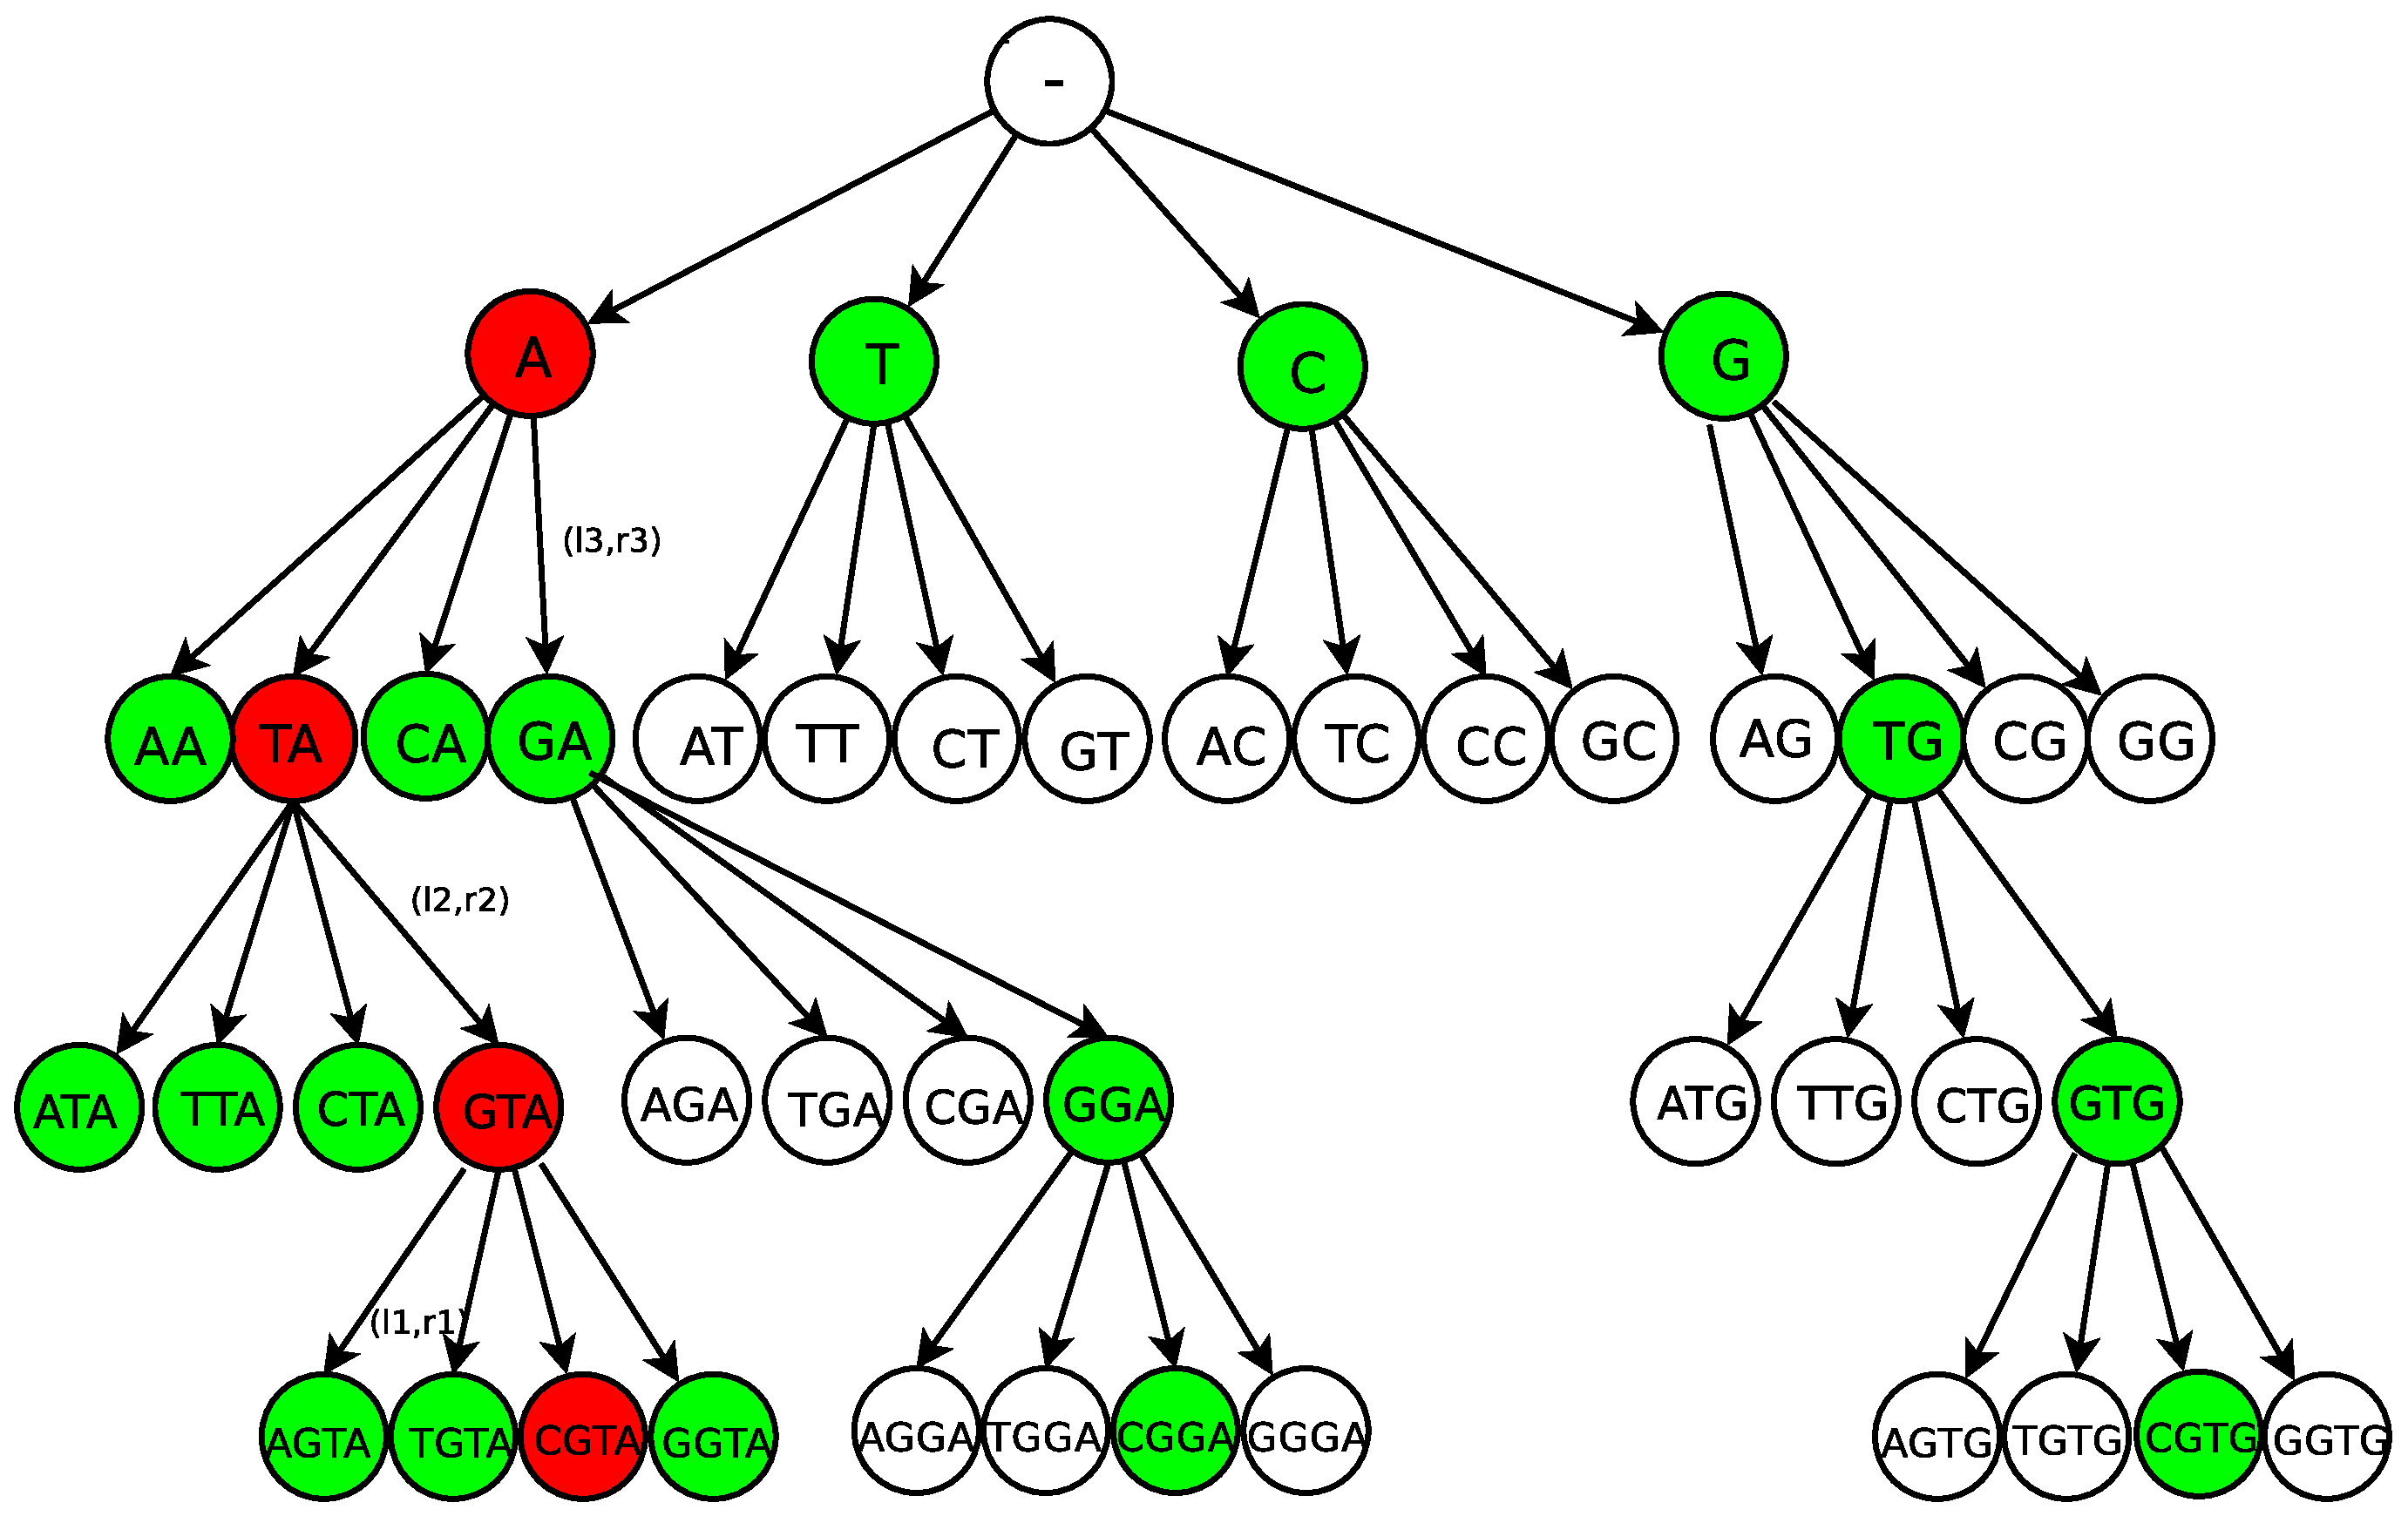
\includegraphics[width=0.9\textwidth]{searchtree.eps}
    \caption{近似匹配示例} \label{fig:searchtree}
\end{figure}

实际上,每一次的替换,删除或者插入操作导致的新的近似序列可以看作一个树上的遍历过程。如图\ref{fig:searchtree}所示,对于一个长
为4的短读 $P=$``CGTA''的搜索过程,简化起见,省略了删除和插入操作。首先通过CSA查询$P[3]=$`A'在参考序列上的后缀数组位置。接着把
$P[3]=$`A'分别替换为`T',`C',`G',在CSA上查找替换后的后缀数组位置。图中红色路径标志的是到当前搜索深度没有替换操作的近似串,而
绿色标记的则是到当前深度有一次替换操作的近似串,无色的是有两次以上替换操作的近似串搜索路径。可以看到,随着搜索深度的增加,搜索
的方向急剧扩大,加上还有未画出的删除和插入操作,可能的搜索方向会更多。

搜索树的本质是对每一个可能的近似序列都进行搜索,假设一个短读序列的长度为$m$,DNA序列字符集为4,根据上一小节,总的时间复杂度为$9^{m-1}+\Theta(m\log n)$。
考虑到$m$一般在20到70之间,如果直接采用搜索树来进行近似匹配,搜索规模会非常大而难以在有效时间内实现。实际上也无需比对所有的近
似串,对于某些替换,删除或者插入操作过多的近似串,应该提前抛弃掉,即采用分支限界法来对搜索树进行剪枝,去除掉无效的搜索方向,降
低搜索空间。

\subsection{分支限界}

根据上一小节的分析,搜索树的搜索空间复杂度是随短读序列长度指数级增长的,因此必须进行适当的剪枝,抛弃一些没有价值的搜索方向。
传统的DNA序列比对中用到了编辑距离(Edit Distance),汉明距离(Hamming Distance)等来度量两个序列的相似度。在此我们也可以使用类
似的方法做分支限界,比如采用编辑距离,可通过给定一个允许的最大编辑距离$maxDistance$,当在短读序列$P$上后向搜索进行到第$i$步
时,在某个搜索方向上的一个近似序列为$P^{'}$,计算$P$和$P^{'}$之间的编辑距离,若距离大于预先定义的$maxDistance$,则抛弃这个搜
索方向,否则,保持这个搜索方向。汉明距离做分支限界的方法和编辑距离方法类似。

采用编辑距离和汉明距离的方法必须对每一个得到的近似序列和短读序列计算距离,这一方面会导致算法效率的降低,另一方面由于我们在做
短读比对时,会有大量的短读需要比对,这些短读的长度不一定都相同,指定唯一的$maxDistance$是不合适的。对此,在论文\cite{li2009fast}
中,作者提出了一种类似于编辑距离的算法,称之为$difference$数组,该算法很好的实现了自适应的类编辑距离的最大限制距离。因此本文
提出的CSAA比对算法也使用$difference$数组作为分支限界的一个条件。$difference$数组是利用$CSA$上的精确匹配算法,首先对需要比对的
短读做预处理,处理过程如算法\ref{alg:darray}所示。处理过的$difference[i]$反映了在搜索$P[i\ldots n-1]$时可以允许的最大替换,插
入,删除操作的次数。由于在序列比对中我们采用的是后向搜索的过程,所以在计算$difference$数组时,也需要从后往前算,使得$difference$
是一个递减的序列,也即在从后往前比对短读$P[0\ldots n-1]$时,越往前,允许的替换,插入,删除数量越多。

\begin{algorithm}
    \caption{计算$difference$数组}
    \label{alg:darray}
    \begin{algorithmic}[1]
        \Require $\Phi,\alpha,\beta,P$
        \Ensure $difference[0\ldots |P|-1]$
        \Function{CalculateDifference}{$\Phi,\alpha,\beta,P$}
            \State $z \gets 0$
            \State $l \gets 0$
            \State $r \gets |P|-1$
            \For{$i \gets |P|-1$ downto $0$}
                \State $(l,r) \gets$ \Call{ExactMatch}{$\Phi,\alpha,\beta,l,r,P[i]$} \Comment{调用算法\ref{alg:exac}}
                \If {$l>r$}
                \Comment{失配,$difference[i]$增加一次,否则$difference[i]$不变}
                \State $l\gets 0$
                \State $r \gets |P|-1$
                \State $z \gets z+1$
                \EndIf
                \State $difference[i] \gets z$
            \EndFor
        \EndFunction
    \end{algorithmic}
\end{algorithm}

$difference$数组的作用,是结合每一个近似序列的一个辅助值$z$来分支限界的。开始比对时,序列$P$的$z$值是$0$,之后每做一次插入,
删除或者替换,则$z$增加一次,而在该操作位置的最大允许删除,插入,替换操作数是$difference[i]$。比较两者,若$z>difference[i]$
则证明该搜索方向做了过多的替换,删除,插入操作,短读已经和参考序列相似度太小,应当删除该搜索方向,考虑搜索树上的其他方向。

除了$difference$距离,另一可用的分支限界策略是罚分机制\cite{lesk1e21986alignment}。在搜索树上向前搜索时,每一次替换,删除或者插入操作都会产生一个新的近
似序列,而每增加一次这样的操作,都会导致这个方向上的近似序列和参考序列的相似度下降。基于此,我们可以预定义一个罚分上限$maxPenalty$。
同时为替换,插入,删除三种操作分别定义各自的罚分,当这个短读比对过程中每做一次上述操作时,都会对这个近似序列增加相应的罚分,
当罚分达到预定义的最大罚分$maxPenalty$时,即认为这个近似序列已经和短读序列相似度太小,没有必要再继续搜索这个方向。通过这样的
罚分机制,可以去除较差的近似序列,达到分支限界的目的。

在生物信息学领域,每一个删除或者插入统称为一个indel,而每一个indel都会在短读序列上造成一个空位(gap),对应的罚分称为空位罚分。
gap通常分为两种,一种是单独出现在序列中,称为gap open;另一种是连续的gap,称为gap extension。gap open的罚分是各个gap罚分的线
性叠加和,而通常gap extension的罚分不能简单的做线性增加来处理。Affine gap penalties\cite{eddy1998profile}是生物信息学领域常用的一种罚分机制,假设
有一个gap extension长为$x$,则这个gap的罚分为$-(\rho +\sigma x)$,其中$\rho >0$,$\sigma$是每一个indel操作的罚分。

有了$difference$距离和$gap$罚分两种分支限界的策略,可以大大减少搜索的规模,通过控制合适的$maxPenalty$可以实现在比对时间和比对
精度之间的平衡。然而如果直接依赖算法\ref{alg:inexact}实现比对算法也是不合适的。因为算法\ref{alg:inexact}是一个递归的算法,递
归算法本身在实际实现时过于低效,我们的short read一般都长30bp以上,这样的深度是不能用递归的。另一方面,递归比对的本质在
搜索树上表现为一个深度优先的搜索,每一次递归都会把一个方向上的所有方向做一次尝试,直到遇到分支限界条件不合适才会回溯到上一层。
这一特性会引起过度回溯的问题。这一问题的本质是每次进入一个新的搜索方向时没有做出正确的选择,整体的搜索方向是随机的,算法大多
数的递归选择都会进入不是最好的方向,从而最终不得不回溯,这显著增大了时间开销。据此本文提出一种优先堆结构,把搜索树上的深度优
先搜索改为广度优先搜索。每一层上都把所有的搜索方向排序放在一个优先堆里,算法每进入下一个搜索方向都在当前优先堆中选择最优的即
罚分最低的搜索方向进入。借助这一优先堆结构,可以把搜索方向限制在只沿着最优的搜索方向前进,从而实现最优比对。同时,还可以限定
优先堆的大小,抛弃掉虽然符合分支限界条件但相对于其他搜索方向过差的搜索方向。

优先队列使用了最大堆来实现,每一项保存一个近似匹配的序列相关匹配信息,以每个近似序列的罚分和$z$值作为优先堆的$key$值。本文中
使用的优先堆支持如下操作:

\begin{itemize}
    \item INIT-HEAP$(heap)$:初始化优先堆$heap$为空。
    \item INSERT-HEAP$(heap,x)$:把元素$x$插入优先堆$heap$中,并按照罚分排序。
    \item EXTRACT-MIN$(heap)$:去掉并返回$heap$中罚分最小的元素。
    \item HEAP-SIZE$(heap)$:返回$heap$中元素的数量。
    \item HEAP-DROP-MAX$(heap)$:删除$heap$中罚分最大的算素。
\end{itemize}

综上所述,我们提出本文的核心比对算法\ref{alg:alignment},该算法中使用了算法\ref{alg:process},后者是在给定的位置上做替换,
插入,删除操作的过程。比对算法\ref{alg:alignment}可以指定$maxPenalty$和$maxHeapSize$两个参数来控制比对的精度和比对时间之间的
平衡。

\begin{algorithm}
    \caption{处理替换,删除,插入}
    \label{alg:process}
    \begin{algorithmic}[1]
        \Require $P,\Phi,\alpha,\beta,x,heap$
        \Ensure $heap$
        \Function {ProcessIndel}{$P,\Phi,\alpha,\beta,x,heap$}
        \State $y.l\gets x.l$;$y.r\gets x.r$;$y.i\gets x.i-1$  \Comment{删除$P[i]$}
        \State $y.penalty \gets x.penalty+delPenalty$
        \State $y.z\gets x.z+1$
        \State \Call{Insert-Heap}{$heap$,$y$}
        \ForAll{$c \in \{A,C,G,T\}$}
            \State $(l,r)\gets$\Call{ExactMatch}{$\Phi,\alpha,\beta,x.l,x.r,c$}
            \If {$l\leq r$}
                \State $y.l\gets l$;$y.r\gets r$;$y.i\gets x.i$ \Comment{在$P[i]$之后插入$c$}
                \State $y.penalty\gets x.penalty+insPenalty$;
                \State $y.z \gets x.z+1$
                \State \Call{Insert-Heap}{$heap,y$}
                \If {$P[i]=c$}  \Comment{match}
                    \State $y.l\gets l$;$y.r\gets r$;$y.i\gets x.i-1$
                    \State $y.penalty\gets x.penalty$;
                    \State $y.z\gets x.z$
                    \State \Call{Insert-Heap}{$heap,y$}
                \Else   \Comment{替换$P[i]$}
                    \State $y.l\gets l$;$y.r\gets r$;$y.i\gets x.i-1$
                    \State $y.penalty\gets x.penalty+subPenalty$
                    \State $y.z\gets x.z+1$
                    \State \Call{Insert-Heap}{$heap,y$}
                \EndIf
            \EndIf
        \EndFor
        \State \Return $heap$
        \EndFunction
   \end{algorithmic}
\end{algorithm}

\begin{algorithm}
    \caption{CSA比对算法}
    \label{alg:alignment}
    \begin{algorithmic}[1]
        \Require $\Phi,\alpha,\beta,P,maxPenalty,maxHeapSize$
        \Ensure $result$    \Comment{输出为符合比对条件的所有结果组成的优先堆}
        \Function{CSAAlignment}{$\Phi,\alpha,\beta,P,maxPenalty,maxHeapSize$}
        \State $difference\gets$\Call{CalculateDifference}{$\Phi,\alpha,\beta,P$}
        \State $heap \gets$ \Call{Init-Heap}{$heap$}
        \State $result \gets$\Call{Init-Heap}{$result$}
        \State $x.l\gets 0$;$x.r\gets |P|-1$;$x.i\gets |P|-1$
        \State $x.penalty\gets 0$;$x.z\gets 0$
        \State $heap\gets$ \Call{ProcessIndel}{$P,\Phi,\alpha,\beta,x.heap$}    \Comment{处理$P[m-1]$}
        \While{$x\gets$\Call{Extract-Min}{heap}}
            \If {$x.i<0$}
                \State \Call{Insert}{$result,x$}    \Comment{获得一个较好的比对结果}
                \State continue
            \EndIf
            \If{$x.z>difference[x.i]$ or $x.penalty>maxPenalty$}  \Comment{剪枝}
                \State continue
            \EndIf
            \State $heap\gets$\Call{ProcessIndel}{$P,\Phi,\alpha,\beta,x,heap$} \Comment{处理$P[0\ldots m-2]$}
            \While{\Call{Heap-Size}{$heap$}>$maxHeapSize$} \Comment{去除较差的比对方向}
                \State \Call{Heap-Drop-Max}{$heap$}
            \EndWhile
        \EndWhile
        \State \Return $result$    \Comment{返回所有符合条件的比对结果}
        \EndFunction
    \end{algorithmic}
\end{algorithm}


\section{CSAA的实现}

上文中给出了CSAA的算法过程,实际实现中CSAA采用了一些优化措施,进一步提高程序的效率。这些措施主要是从提高执行效率和准确度
两个方面来考虑的。CSAA主要包括三个子程序:build index,alignment,output。build index子程序完成对参考序列$T$建立压缩后缀数组
索引,对同一个参考序列只需建立一次索引即可。alignment子程序是CSAA的核心,完成对短读序列到参考序列$T$的映射,输出CSAA
自定义的一种SAI格式文件。最终SAI格式文件通过output子程序转为标准比对结果文件SAM(Sequence Alignment/Map format)。

\subsection{使用seed提高比对速度}
在DNA测序技术中,单端测序和双端测序都存在测序质量的问题。离引物结合位点越近的位置,测序结果准确率越高,而越远的位置,测序准确率
越低。根据这一现象,关于Bowtie实现的论文\cite{langmead2009ultrafast}中提出了seed的概念,该论文认为针对短读序列中测序可信度较高
的部分采用较高的限制,在较低的地方做较低的限制可以取得更快的比对速度和更好的比对结果。如图\ref{fig:seed}所示,read前面绿色部分
是可信度比较高的seed部分,后面是可信度比较低的非seed部分。

\begin{figure}[htbp]
    \centering
    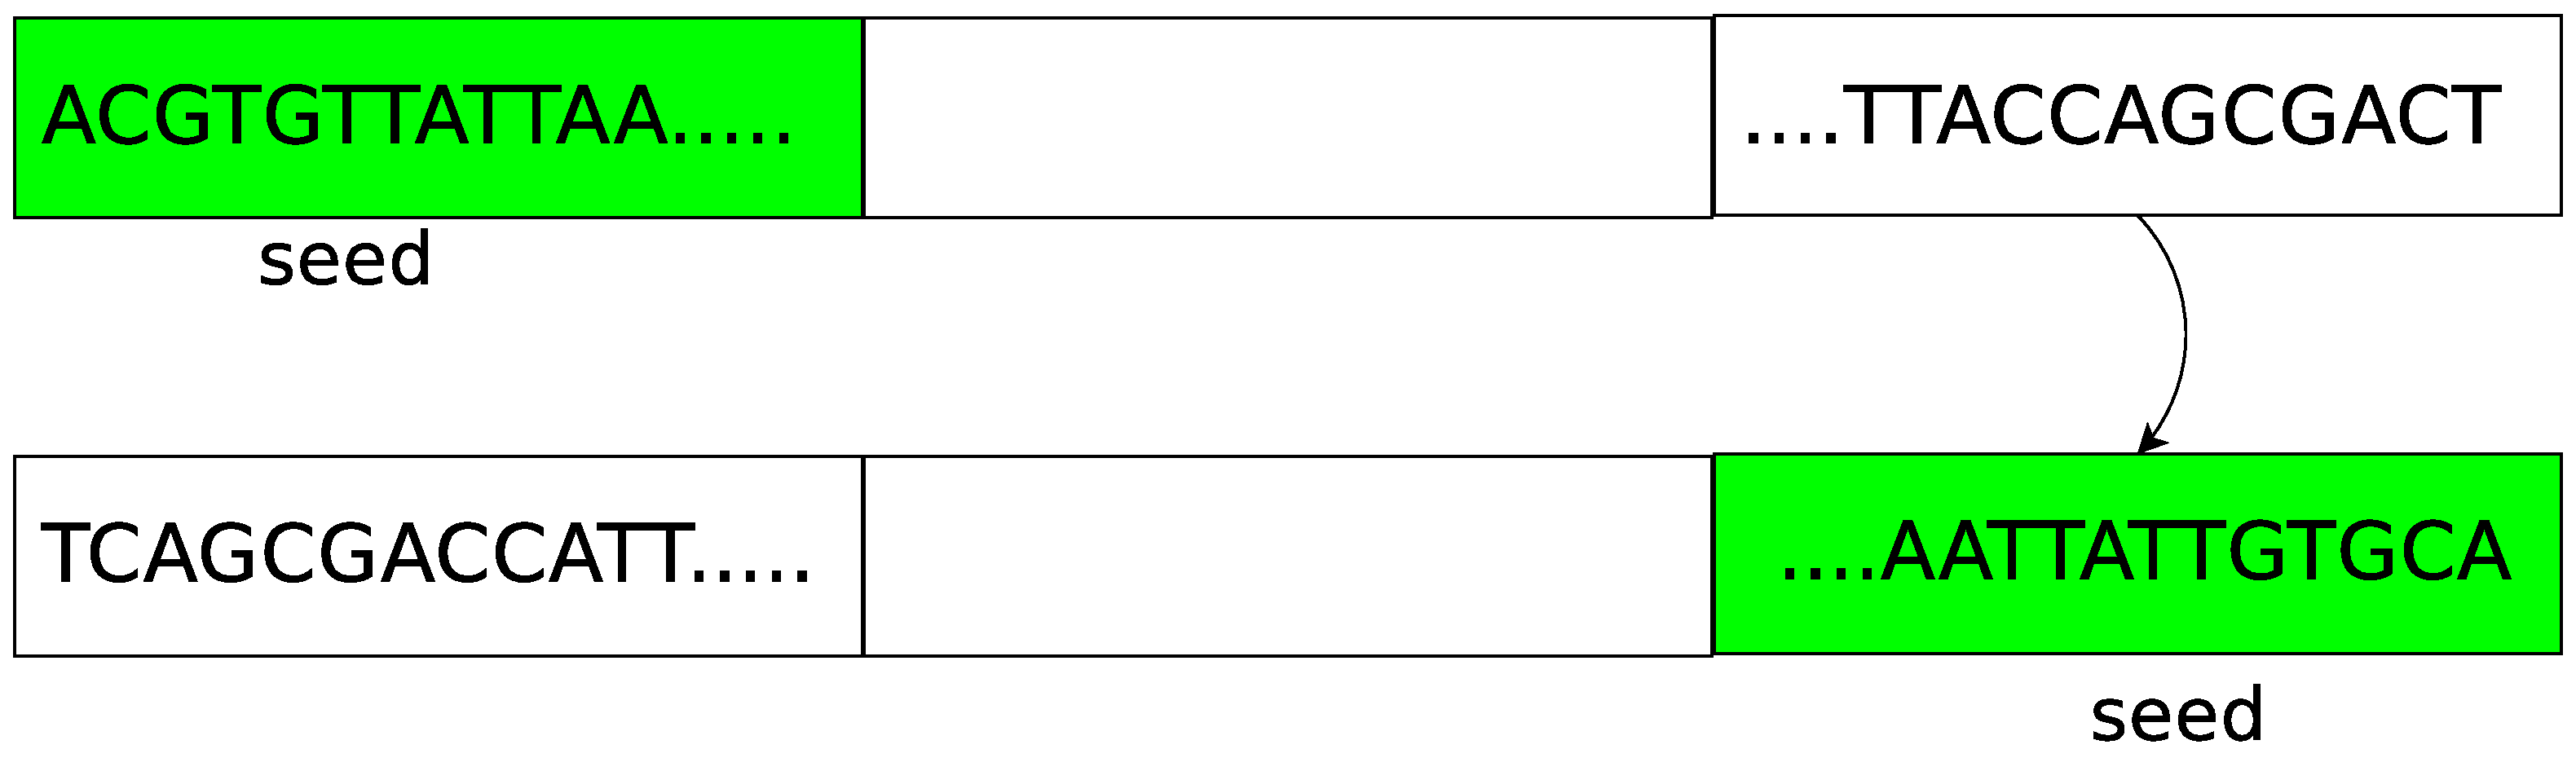
\includegraphics[width=0.9\textwidth]{seed.eps}
    \caption{seed示例} \label{fig:seed}
\end{figure}

在算法\ref{alg:alignment}中,我们当某个近似序列的$x.penalty>maxPenalty$时,会直接剪枝。CSAA中实际上是分为两部分来剪枝的,seed部有
一个$maxPenalty$,非seed部分有另一个$maxPenalty$,前者较小,后者较大。通过这样的策略,可以控制搜索结果中的待选近似序列中的替换
删除,插入等操作的绝大部分发生在非seed部分,即read的不可靠部分,从而有效提高比对的精度。至于seed的具体长度,可以根据不同的测序
技术来给定。默认情况下,Bowtie的seed长度是28,随本文发布的CSAA中seed的默认长度是32。

因为seed的限制条件较高,所以如果能首先对seed进行匹配,可以尽早抛弃掉一些不满足seed部分匹配要求,从而不用搜索非seed部分,从而
提高搜索速度。但因为seed是在短读序列的前缀部分,而我们使用CSA索引的后向搜索时是从后往前搜索的,最后才搜索seed部分。所以在CSAA中无论是建
立索引还是短读匹配都是对短读的逆序序列进行的。如图\ref{fig:seed}所示,通过逆序,把read的seed部分转到后向搜索的首先搜索的部分。

在图\ref{fig:seedaccuracy}中,对seed的长度对比对速度和比对精度做了对比测试,测试中的数据同图\ref{fig:alignment}使用的模拟数据相同,
都是100万条hg19上的仿真数据,indel概率为0.01\%,SNP概率为0.09\%,不同的是本次实验中只测试了长为70bp的短读。可以发现,seed的选
取对比对速度有着明显的影响,seed选取的越长,比对的速度越快,几乎成线性下降的趋势。seed的长度对recall rate和accuracy同样有影响,
seed选取的越长,recall rate有明显下降,这是因为如果seed越长,seed部分不匹配的可能越大,造成更多的短读不能匹配到参考序列上,而
accuracy有所提高则是因为较长的seed选取,抛弃了更多的可能错误匹配,保证了更少的匹配错误。

\begin{figure}[htbp]
    \centering
    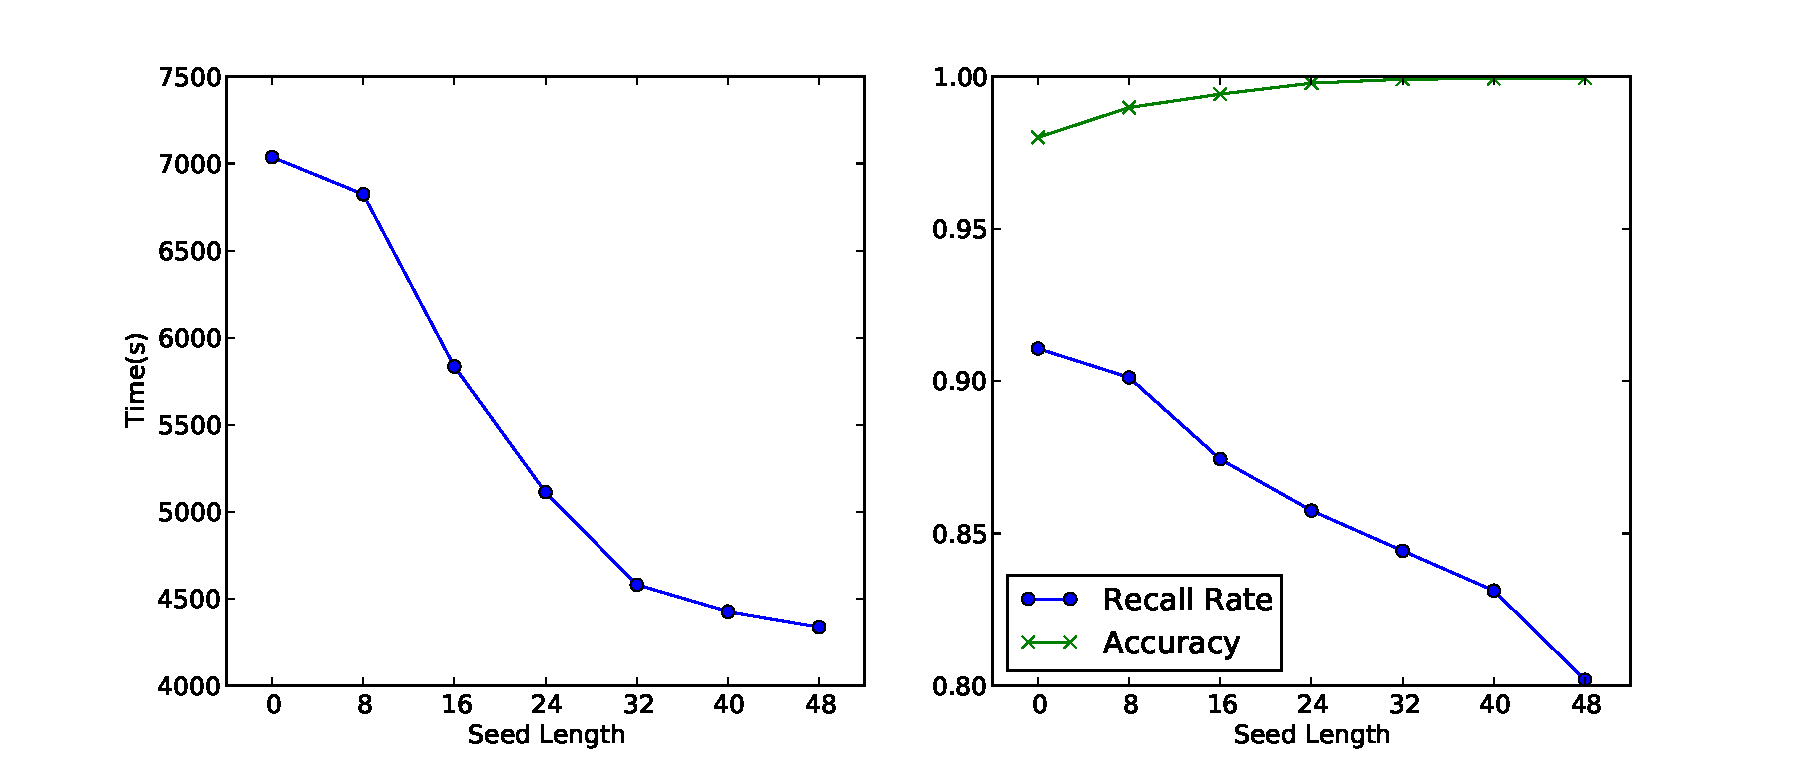
\includegraphics[width=1.1\textwidth]{seedaccuracy.pdf}
    \caption{seed长度对比对速度和比对精度的影响} \label{fig:seedaccuracy}
\end{figure}


本文中,比对精度包括两个测量指标,一个是recall rate,一个是mapping accuracy。recall rate是正确比对的短读(correctly mapped reads)
数占总的短读数(all reads)的比例,而mapping accuracy是正确比对的短读数(correctly mapped reads)占成功比对到参考序列上的短读(mapped reads)
的比例。在序列比对中,对于实际测序实验中得到的短读数据,由于预先并不知道短读的真正位置,所以正确比对的短读(correctly mapped reads)
数量是未知的。只有用模拟数据才能获取短读的真正位置,再用比对软件对模拟生成的短读进行比对,把获取的比对结果和预知的模拟短读的真正
位置做比较就能度量该比对软件的正确比对短读数目,从而计算出mapping accuracy,来度量一个软件的比对的可信度。另一方面,因为比对软件
在比对中设定的一些参数限制,如本文中的罚分,difference距离等等,使得一些发生了较大的变异(SNP,indels)的短读不能映射到参考序列上,
即该短读没有映射位置,从而造成最终在所有短读中只有一部分得以映射到参考序列上,这就是mapped reads,而recall rate即反映了这一衡
量短读比对性能的指标。在实际比对中,比对软件得到的参考序列上的比对位置和生成仿真数据时的实际位置并不需要完全比上,只要二者之间
的距离在一定距离内即认为这个比对结果是正确的,本文中所有的实验中这一距离定义为20。

\subsection{比对过程并行化}
CSAA给参考序列建立索引需要很多时间,但我们只需要给一个参考序列建一次索引就可以了,其后的向同一参考序列的比对无需再建立一次
索引。在比对阶段,由于一次实验的短读数量非常大,通常在几百万到数十亿条的规模,这使得比对过程通常耗时非常长。

观察比对的过程可以发现,每一条短读的比对都是独立进行的,之间互相只共享参考序列索引的数据和操作,且比对结果也是互相独立的一个
优先堆。据此,我们可以很容易的设计一个并行计算的算法来完成比对。考虑到在计算过程中需要共享参考序列索引以及匹配算法的操作。所以
CSAA选择了多线程编程模型作为并行方案。

csaa在执行比对时,可以指定线程的数量,程序启动后,将建立多个线程,并把所有的短读数据分成多份,由每个线程单独执行一份,从而实现
快速的比对。每个线程比对完成后都会把比对结果写如一个临时文件,待所有的线程执行完毕后再按顺序把比对结果输出到程序指定的文件。
具体的并行算法如算法\ref{alg:mt}所示。

\begin{algorithm}
    \caption{CSAA比对并行算法}
    \label{alg:mt}
    \begin{algorithmic}[1]
        \Require $k,\Phi,\alpha,\beta,maxPenalty,maxHeapSize$
        \Ensure $result$
        \Function{Match-MULT}{$k,\Phi,\alpha,\beta,maxPenalty,maxHeapSize$}
        \State 分割reads文件为$k$个小文件$\{read_1,read_2 \ldots read_k \}$
        \State 建立$k$个线程$threads=\{thread_1,thread_2\ldots thread_k\}$
        \ForAll{$thread_i \in threads$ }
            \State 从文件$read_i$读取一个短读$read$
            \State \Comment{调用算法\ref{alg:alignment}}
            \State $result \gets $\Call{CSAAlignment}{$\Phi,\alpha,\beta,read,maxPenalty,maxHeapSize$} 
            \State 输出$result$到文件$result_i$
        \EndFor
        \State 合并文件$\{result_1,result_2\ldots result_k\}$到文件$result$
        \State 输出文件$result$
        \EndFunction
    \end{algorithmic}
\end{algorithm}

通过增加比对时的线程数量可以快速减少比对的时间,如图\ref{fig:alignment}所示。实验中所用的参考序列为来自NCBI的人类基因组
hg19.fa,短读序列是用wgsim仿真程序生成的模拟短读数据,短读长分别为35bp,70bp,125bp,0.09\%的SNP出现几率,0.01\%的indel出现几率,
短读数量为100万个。可以看到,当由单线程变为双线程时,比对时间减少了一倍,这显示CSAA的多线程能明显提高比对的速度。之后再提高
线程数不能再提高比对速度是因为测试机器是双核的,再多的线程已经不能有效提高CSAA的比对速度。对应的,当进程数增多时,比对所需要
的内存也随之增多。图\ref{fig:alignment}中的曲线还显示,比对的速度以及内存消耗和短读长是密切相关的,短读越长,比对的时间也
越长,所需内存也越多。

\begin{figure}[tbp]
    \centering
    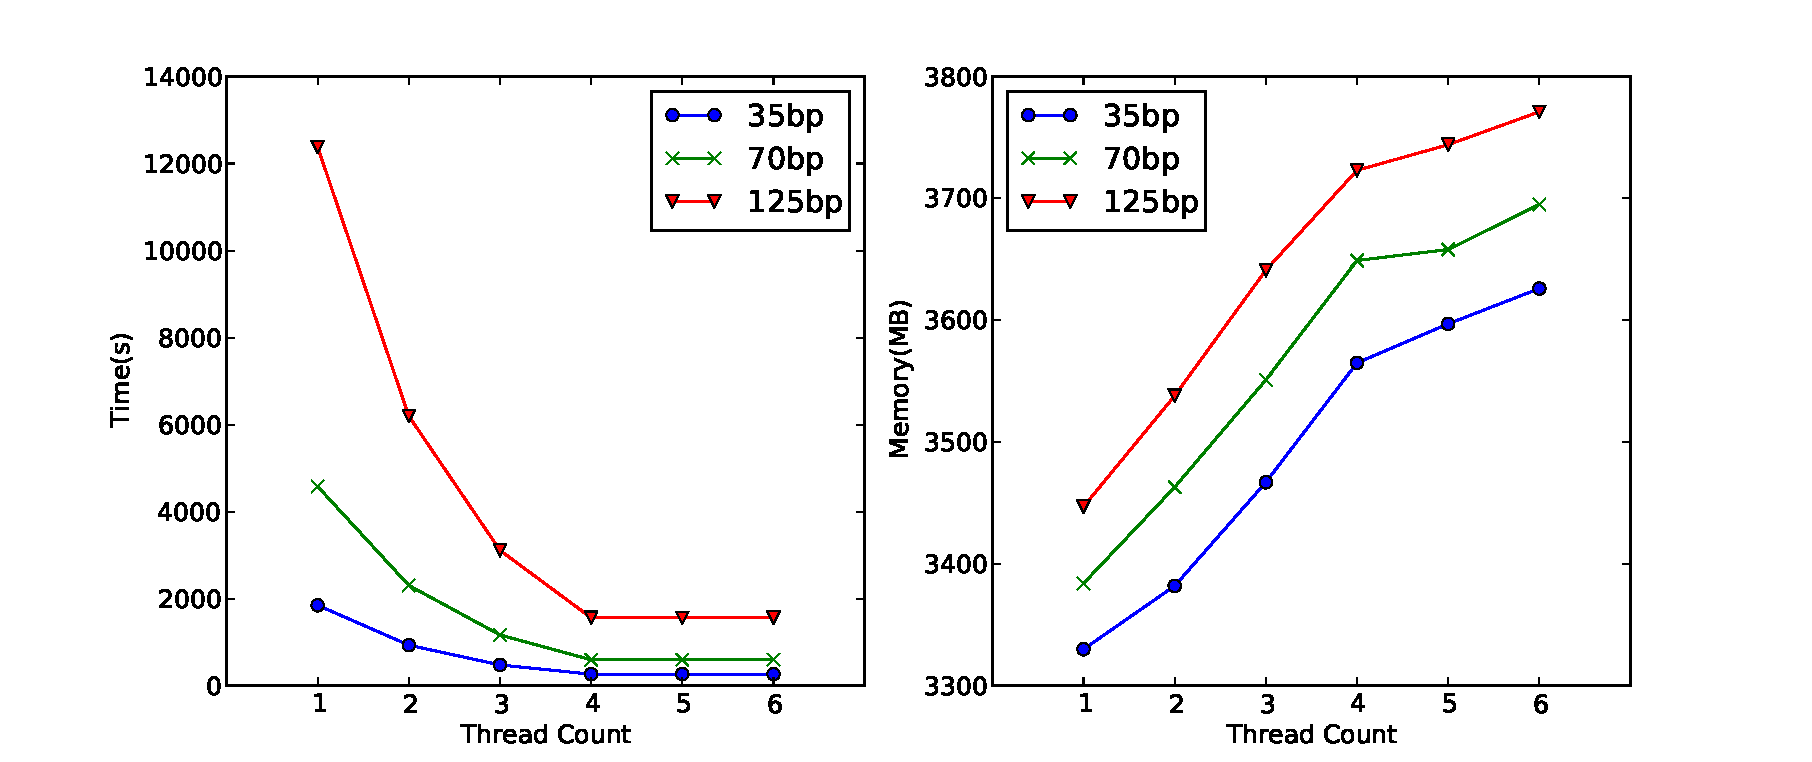
\includegraphics[width=1.1\textwidth]{alignment.pdf}
    \caption{多线程比对的时间空间效率} \label{fig:alignment}
\end{figure}

\section{实验测试}

为测试CSAA的性能,本文同时测试了Bowtie\cite{langmead2009ultrafast}和BWA\cite{li2009fast}这两个个比对工
具的性能,以和CSAA进行比较。分别对比这几个工具在不同规模数据上建立索引时的时间,需要的内存;以及在模拟数据上和真实数据上的比对能力。
这三个工具中,Bowtie和BWA是用基于BWT的索引建立
的比对工具,其中Bowtie采用了回溯法实现替换操作,但不支持insert和delete操作,即上文中所论述的gap alignment。BWA除了支持insert,
delete之外,还加入了Smith-Waterman方法提高比对精度。此外Bowtie和BWA和我们的CSAA都支持多线程比对,但在比对测试中,我们的csaa和bwa,
bowtie等都只使用单线程运行。

\subsection{测试环境和数据}

在对CSAA的对比测试中,我们使用gcc 4.8编译链接CSAA,并且使用了-O3优化。系统环境为64位redhat 5.0,测试机器有64GB内存和24
核CPU。测试使用的数据是标准的人类基因组序列,ucsc version为hg19,来自1000 Genome Project的名为Genome Reference Consortium GRCh37
的参考序列。实验中所用的模拟数据也是在该数据上生成。

测试中,CSAA和BWA在测试时均指定单线程,seed长为32。Bowtie使用的是Bowtie-v1,使用单线程,使用--best -k 2参数。
Bowtie使用长为32的seed。模拟数据的获取和比对精度结果获得中使用了SAMtools系列工具中的wgsim和wgsim-eval。

\subsection{索引建立时间}
表\ref{tab:tab1}中对比了bowtie,BWA和CSAA三种工具分别建立索引时所需要的时间和内存消耗对比情况,表中数据分别对应几个工具在索引
512M,1024M和2048M的数据时所需要的时间和内存。CSAA中使用经典方法构建压缩后缀数组。

\begin{table}[htbp]
    \caption{建立索引的时间空间对比}
    \label{tab:tab1}
    \centering
    \begin{tabular}{lrrrp{2ex}rrr}
        \hline
        \multirow{2}{*}{Program} & \multicolumn{3}{c}{Time(m)}& & \multicolumn{3}{c}{Memory(MB)}\\
        \cline{2-4}
        \cline{6-8}
        & 512M &1024M &2048M& &512M &1024M &2048M\\
        \hline
        Bowtie&21.85 &45.33 &93.02& &987 &1109 &1210 \\
        BWA&7.85 &16.33 &34.72& &1890 &1902 &2006 \\
        CSAA&6.27 &14.0 &29.87& &2113 &8680 &19532 \\
        \hline
    \end{tabular}
\end{table}

从表\ref{tab:tab1}中的测试结果可以看到,CSAA相对其他两个比对工具在索引时间上具有较大优势。其中Bowtie建立索引时是分块建立索引
的,最终再合并成一个索引,时间效率最差,但需用内存空间最小。

\subsection{模拟数据测试}
本文使用SAMtools工具包中的wgsim工具从人类基因组序列hg19中随机生成模拟的短读序列。然后,分别用四种比对工具对这些模拟的
短读序列进行比对,最后测试比对速度以及比对精确度。因为这些模拟数据在参考序列上的映射位置是已知的,所以可以计算出各个工具的比
对结果的accuracy。本次实验中的精度测试工具使用SAMtools中的wgsim\_eval.pl程序。

表\ref{tab:singleend}和\ref{tab:pairend}所示为四个测试工具在单端和双端模拟数据上的的比对结果展示,参考序列是人类基因组序列
hg19,模拟短读序列的长度为70bp,总共有100万个短读。

表\ref{tab:singleend}和\ref{tab:pairend}中的实验的模拟数据使用wgsim程序在人类基因组上生成的短读长为70的模拟数据,生成过程中,单核苷酸变
异(SNP)的概率是0.09\%,indel变异的概率是0.01\%,生成双端模拟数据时的fragment distance的长度满足正太分布$N(500,50)$。对比结果
中Rec是recall rate,Acc是accuracy。意义如上文中所解释。从表中可以看出,CSAA相对于BWA和Bowtie在查询时更节省内存,在recall rate
和accuracy上和BWA,Bowtie基本持平。%出现这样的结果是因为BWA和CSAA都支持indel操作,而Bowtie则只支持substitution操作,当短读序列比
%较长时其比对效果就会下降。

\begin{table}[htbp]
    \caption{单端模拟数据比对测试}
    \label{tab:singleend}
    \centering
    \begin{tabular}{lrrrr}
       \hline \\
       Program&Time&Memory(M)&Rec(\%)&Acc(\%)\\
       \hline \\
       Bowtie&24m38s&2923&80.21&98.64\\
       BWA&39m57s&3506&89.32&99.91\\
       CSAA&1h16m20s&3384&84.44&99.91\\
       \hline\\
    \end{tabular}
\end{table}


\begin{table}[htbp]
    \caption{双端模拟数据比对测试}
    \label{tab:pairend}
    \centering
    \begin{tabular}{lrrrr}
       \hline \\
       Program&Time&Memory(M)&Rec(\%)&Acc(\%)\\
       \hline \\
       Bowtie&26m29s&2931&83.47&98.67\\
       BWA&43m25s&4954&94.71&99.97\\
       CSAA&1h17m55s&4023&88.57&99.97\\
       \hline\\
    \end{tabular}
\end{table}

\subsection{真实数据测试}
为测试CSAA在真实数据上的表现,本文从网络上下载了12.2 million个长为51bp的短读数据库。这些数据来自European Read Archive
(AC:ERR000589),是1000 Genomes Project的一个名男性基因组测序,由Illumina测序技术完成测序。参考序列选的是人类基因组,
测序编号hg19。由于真实数据的比对位置并不能事先获取,所以在测试真实数据时使用Mapped rate来度量比对效果。Mapped rate
指比对程序在指定参数条件下能够给出比对结果的短读数目和所有测试数据中短读数目总和的比例。在本次比对中测试中,Bowtie,BWA和
CSAA使用默认的长为32的seed策略,Bowtie使用--best -k 2参数。

\begin{table}[htbp]
    \caption{实际数据比对测试}
    \label{tab:tab3}
    \centering
    \begin{tabular}{lrrrr}
       \hline\\
       Program&Time&Memory(MB)&Mapped(\%)&Paired(\%)\\
       \hline\\
       Bowtie&3h48m47s&2929&75.2&83.75\\
       BWA&3h4m24s&4845&87.67&99.83\\
       CSAA&6h49m17s&4008&83.18&99.75\\
       \hline\\
    \end{tabular}
\end{table}

表\ref{tab:tab3}中的测试结果显示,在实际数据中CSAA也具有较高的准确性,84\%的短读序列都能映射到参考序列上,
基本性能和BWA很接近。在时间方面,CSAA,BWA,Bowtie都使用索引参考序列再比对的方法,而MAQ则使用了索引短读序列的方法,所以
CSAA,BWA,Bowtie的比对时间都比较接近,Bowtie能更快一些。在比对使用的空间上,相对而言,CSAA使用了更少的内存,空间效率
优于其他三种发放,在常规PC机上具有优势。

\section{总结}
本文提出了一种基于压缩后缀数组的短读比对算法,利用CSA的后向搜索实现了近似匹配,结合搜索树和优先堆,最终提出了一种高效准确
的短读比对算法。该算法和主流的短读比对算法相比,准确性更高,且使用更少的内存,在准确率和空间高效方面达到很好的权衡。

\bibliographystyle{plain}
\bibliography{reference}
\end{document}
